\section{MIP model}
Malapert's original MIP approach, as given in Model \ref{model:malapertmip},
uses a set of binary decision variables $x_{jk}$ to represent whether job $j$ is
assigned to batch $k$. The original model assumes a set $K$ of $|K| = |J|$
batches, the number of jobs being a trivial upper bound on the number of
batches required; it also enforces an earliest-due-date-first (EDD) ordering of
the batches (constraint \ref{c:malapp-edd}).
\begin{model}[h]
\begin{alignat}{2}
\mathrm{Min.}\quad & \Lmax && \\
\mathrm{s.t.}\quad &\sum_{k \in K} x_{jk} = 1 \quad && \forall j \in J \\
  &\sum_{j \in J} s_j x_{jk} \leq b \quad && \forall k \in K\\
  &p_j x_{jk} \leq P_k \quad && \forall j \in J, \forall k \in K\\
  &C_{k-1} + P_{k} = C_k \quad && \forall k \in K\\
  &(d_{max} - d_j)(1 - x_{jk}) + d_j \geq D_k \quad && \forall j \in J, \forall k \in K\\
  &D_{k-1} \leq D_k \quad && \forall k \in K \label{c:malapp-edd} \\
  &C_k - D_k \leq \Lmax \quad && \forall k \in K\\[2ex]
  &C_k \geq 0, P_k \geq 0 \text{ and } D_k \geq 0 \quad && \forall k \in K  
\end{alignat}
\caption{Malapert's original MIP model}
\label{model:malapertmip}
\end{model}

\section{Improved MIP model}
\subsection{Grouping empty batches}
The given formulation lacks a rule that ensures that no empty batch is followed by a non-empty batch. Empty batches have no processing time and a due date only bounded by $d_\text{max}$, so they can be sequenced between non-empty batches without negatively affecting $\Lmax$. Since, however, desirable schedules have no empty batches scattered throughout, we can easily reduce the search space by disallowing such arrangements. The idea is illustrated in Figure \ref{fig:dominancerule}.


\begin{figure}
  \centering
  \begin{subfigure}[b]{0.4\textwidth}
    \centering
    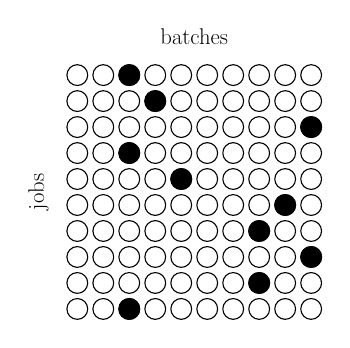
\begin{tikzpicture}[scale=0.33]
      \pgftext[x=-1.5cm, y=4.5cm, rotate=90]{\sansfont\Huge jobs}
      \pgftext[x=4.5cm, y=10.5cm]{\sansfont\Huge batches}

      \foreach \j in {0,...,9}
      {
        \foreach \k in {0,...,9}
        {
          \draw[] (\k, \j) circle [radius=0.4];
        }
      }
      \draw [fill] (2,0) circle [radius=0.4];
      \draw [fill] (2,6) circle [radius=0.4];
      \draw [fill] (2,9) circle [radius=0.4];
      \draw [fill] (3,8) circle [radius=0.4];
      \draw [fill] (4,5) circle [radius=0.4];
      \draw [fill] (7,1) circle [radius=0.4];
      \draw [fill] (7,3) circle [radius=0.4];
      \draw [fill] (8,4) circle [radius=0.4];
      \draw [fill] (9,2) circle [radius=0.4];
      \draw [fill] (9,7) circle [radius=0.4];
    \end{tikzpicture}
    \caption{Without dominance rule}
  \end{subfigure}
  \begin{subfigure}[b]{0.4\textwidth}
    \centering
    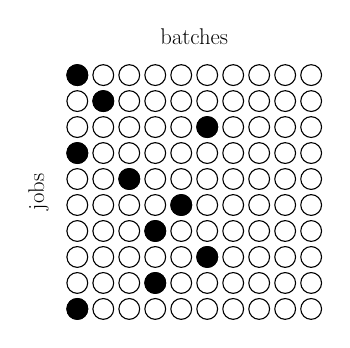
\begin{tikzpicture}[scale=0.33]
      \pgftext[x=-1.5cm, y=4.5cm, rotate=90]{\sansfont\Huge jobs}
      \pgftext[x=4.5cm, y=10.5cm]{\sansfont\Huge batches}

      \foreach \j in {0,...,9}
      {
        \foreach \k in {0,...,9}
        {
          \draw[] (\k, \j) circle [radius=0.4];
        }
      }
      \draw [fill] (0,0) circle [radius=0.4];
      \draw [fill] (0,6) circle [radius=0.4];
      \draw [fill] (0,9) circle [radius=0.4];
      \draw [fill] (1,8) circle [radius=0.4];
      \draw [fill] (2,5) circle [radius=0.4];
      \draw [fill] (3,1) circle [radius=0.4];
      \draw [fill] (3,3) circle [radius=0.4];
      \draw [fill] (4,4) circle [radius=0.4];
      \draw [fill] (5,2) circle [radius=0.4];
      \draw [fill] (5,7) circle [radius=0.4];
    \end{tikzpicture}
    \caption{With dominance rule}
  \end{subfigure}
\caption{Dominance rule to eliminate empty batches followed by non-empty batches
(circles represent the $x_{jk}$ variables; a filled circle stands for $x_{jk} =
1$)}\label{fig:dominancerule}
\end{figure}


A mathematical formulation is
\begin{alignat}{2}
& \sum_{j \in J} x_{j,k-1} = 0 \rightarrow \sum_{j \in J} x_{jk} = 0 \quad && \forall k \in K. \label{eq:emptybatch0}
\end{alignat}

To implement this, we can write constraints in terms of an additional  set of binary variables, $e_k$, indicating whether a batch $k$ is empty or not:

\begin{alignat}{2}
& e_k + \sum_{j \in J} x_{jk} \geq 1 \quad && \forall k \in K, \label{eq:emptybatch1} \\
& n_j (e_k-1) + \sum_{j \in J} x_{jk} \leq 0 \quad && \forall k \in K. \label{eq:emptybatch2}
\end{alignat}

Constraints \eqref{eq:emptybatch1} enforce $e_k = 1$ when the batch $k$ is
empty. Constraints \eqref{eq:emptybatch2} enforce $e_k = 0$ otherwise, since the sum term will never exceed $n_j$. The rule \ref{eq:emptybatch0} can now be expressed as $e_{k-1} = 1 \rightarrow e_k = 1$, and implemented as follows:

\begin{alignat}{2}
& e_k - e_{k-1} \geq 0 \quad && \forall k \in K.
\end{alignat}

We can also prune any attempts to leave the first batch empty by adding a constraint $e_0 = 0$.

{\color{darkred} This, while it works just fine, actually takes longer than without it.}

\subsection{No postponing of jobs to later batches}
Since the jobs are already sorted by non-decreasing due dates, it makes sense to explicitly instruct the solver never to attempt to push jobs into batches with a greater index than their own: even if every job had its own batch, it would be unreasonable to ever postpone a job to a later batch.
\begin{alignat}{2}
  & x_{jk} = 0 \quad && \forall \{j \in J, k \in K | j > k \}
\end{alignat}


